\laborator{Определение фазовой диаграммы вещества на основе аналитического уравнения состояния}

\goal{на основе данных по свойствам вещества в критической точке определить параметры уравнения состояния Ван дер Ваальса; с помощью данного уравнения произвести расчеты фазовой диаграммы и давления насыщенных паров вещества; результаты представить графически.}

\subsubsection{Теория}
Аналитическое уравнение состояния представляет собой соотношение между давлением, температурой и мольным объемом. В настоящее время существует много различных форм такой связи. Одним из первых аналитических уравнений состояний, которое было предложено еще в 19 веке, является уравнение Клапейрона – Менделеева:
\begin{equation}\label{eq:eos.ideal}
	p V= N R T,
\end{equation}
где $p$ --- давление газа; $T$ --- абсолютная температура; $V$ --- объем, занимаемый газом; $R$ --- универсальная газовая постоянная; $N$ --- число молей газа. Данное уравнение называют также уравнением идеального газа. 

Оказалось, что для большинства реальных газов, например $\mathrm{CO_2}$, $\mathrm{N_2}$, $\mathrm{O_2}$, данное уравнение хорошо описывало экспериментально наблюдаемые соотношения между $p$, $V$, $T$ лишь при давлениях до нескольких атмосфер. Кроме того, уравнение \eqref{eq:eos.ideal} становится бесполезным при рассмотрении процесса сжижения газов. Идеальный газ остается газом при всех температурах, его объем можно уменьшать до бесконечно малой величины.
 
Иоханнес Дидерик Ван дер Ваальс (1837–1923 гг.) предложил модификацию уравнения идеального газа, учитывающую особенности реальных газов: влияние сил межмолекулярного взаимодействия и размеры молекул. Межмолекулярное притяжение уменьшает давление по сравнению с тем значением, которое оно имеет для идеального газа, так как силы притяжения между молекулами уменьшают скорость движения молекул, приближающихся к стенкам. Если $p_{real}$ --- давление реального газа, а $p_{id}$ --- соответствующее давление идеального газа, т.е. давление в отсутствие межмолекулярных сил притяжения, то $p_{id}=p_{real}+\delta p$, где $\delta p$ --- поправка, зависящая от плотности числа частиц ($\delta p = a \left(\frac{N}{V} \right)^2$). Объем, занимаемый молекулами, меньше объема контейнера, в который они заключены, так как размеры молекул конечны. Поправка к объему из-за размеров молекул, т.е.  поправка на «исключенный объем», пропорциональна числу молекул, т.е. $V_{id}=V-b N$, где $b$ --- поправка на 1 моль. Модификация уравнения состояния идеального газа \eqref{eq:eos.ideal}, учитывающая силы межмолекулярного взаимодействия предложена Ван дер Ваальсом в 1873 году:
\begin{equation} \label{eq:eos.vdv}
	\left( p+ \dfrac{a N^2}{V^2} \right) (V- Nb) = N R T.
\end{equation}



В этом уравнение постоянная $a$ характеризует силы притяжения между молекулами, а постоянная $b$, пропорциональная размеру молекул, характеризует силы отталкивания, т.е. $a$ и $b$ отражают природу конкретного вещества.

При постоянной температуре $Т$ типичные $p-V$ зависимости, называемые $p-V$~--~изотермами, для газа Ван дер Ваальса представлены на рисунке \ref{fig:eos.vdw}

\begin{figure}[h]
	\begin{center}
		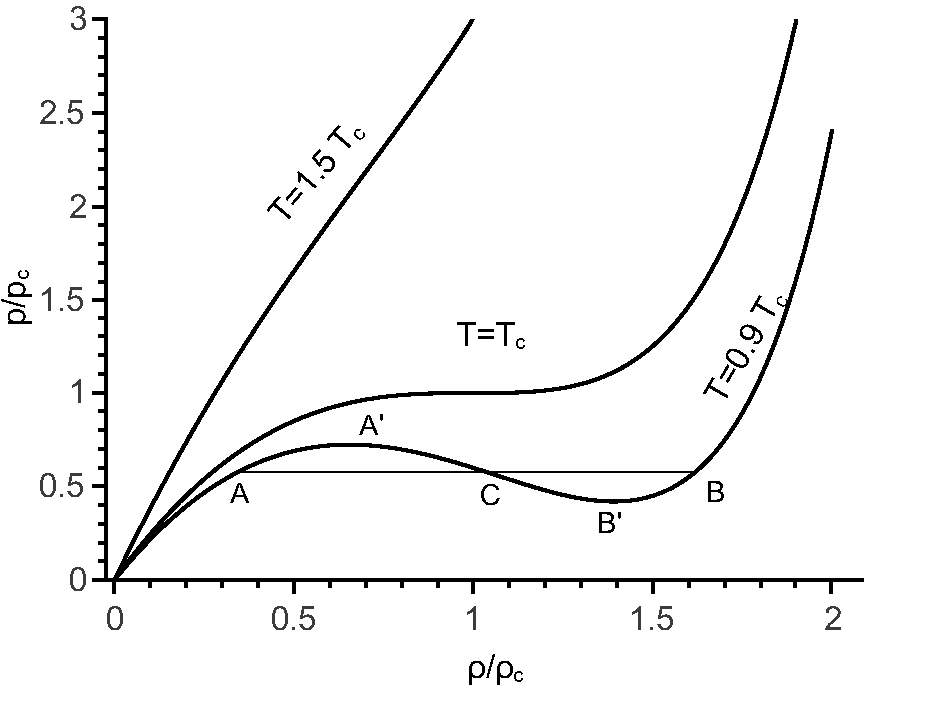
\includegraphics[width=\textwidth]{eos-vdw.pdf}
	\end{center}
	\caption{Изотермы Ван дер Ваальса. При $Т < Т_c$ существует область АА'СВ’В, в которой при заданном давлении $p$ плотность $\rho$ не определяется однозначно уравнением Ван дер Ваальса. В этой области газ превращается в жидкость} \label{fig:eos.vdw}
\end{figure}

Уравнение Ван дер Ваальса свидетельствует о существовании критической температуры $Т_{c}$: при $Т < Т_{c}$ это уравнение описывает кубическую кривую, имеющую два экстремума. В этой области существует фазовый переход пар~-- жидкость. При приближении температуры к $Т_{c}$ эти два экстремума сближаются и, наконец, при $Т=Т_{c}$ сливаются, соответственно переход из газовой фазы в жидкую не происходит, различие между газом и жидкостью исчезает.
При $Т > Т_{c}$ кривая $p-V$ всегда однозначна. Это говорит о том, что в этой области температур не существует перехода в жидкое состояние. Давление и объем, при которых исчезает различие между жидкостью и газом, называют критическим давлением $p_{c}$ и критическим объемом $V_{c}$. Критические параметры $p_{c}$, $V_{c}$ и $Т_c$ могут быть измерены экспериментально и их значения для веществ приведены в справочниках. Критические параметры можно связать с параметрами Ван дер Ваальса $а$ и $b$:
\begin{equation}
	T_{c}=\dfrac{8 a}{27 R b},
\end{equation}
\begin{equation}
	p_{c}=\dfrac{a}{27 b^2},
\end{equation}
\begin{equation}
	{V_m}_{c}=3 b,
\end{equation}
где ${V_m}_{c}$ --- мольный критический объем. Значения постоянных $a$ и $b$ для многих газов приведены в справочной литературе \cite{rid1982}.

Так как для каждого газа существуют свои критические параметры $p_{c}$, $V_{c}$ и $T_{c}$, то это позволяет ввести безразмерные переменные состояния:
\begin{equation}
	T_{r}=\dfrac{T}{T_{c}},
\end{equation}
\begin{equation}
	p_{r}=\dfrac{p}{p_{c}},
\end{equation}
\begin{equation}
	{V_m}_{r}=\dfrac{V_m}{{V_m}_{c}}.
\end{equation}

Если уравнение Ван дер Ваальса записать в приведенном виде, то получится следующее универсальное уравнение, применимое для любых газов:
\begin{equation} \label{eq:eos.vdvb}
	p_r=\dfrac{8 T_r}{2 {V_m}_r-1}-\dfrac{3}{{V_m}_r^2}.
\end{equation}
Уравнение \eqref{eq:eos.vdvb} в большинстве случаев подтверждается экспериментально. Это означает, что приведенные давления всех газов имеют одно и то же значение при заданном приведенном объеме и приведенной температуре. Этот факт получил название закона соответственных состояний. Согласно этому закону, предполагается, что приведенные свойства (приведенное свойство представляет собой отношение свойство / свойство в критической точке) всех газов и жидкостей по существу одинаковы.

В настоящее время существуют более точные уравнения состояния (Редлиха~-- Квонга, Бенедикта~-- Уэбба~-- Рубина и др. \cite{rid1982,yelles1989}), но все же следует отметить, что уравнение Ван дер Ваальса до сих пор полезно для создания хоть и приближенного, но простого аналитического представления о поведении реальных газов и жидкостей.

Наличие уравнения состояния для вещества позволяет производить расчеты термодинамических свойств вещества, в том числе и его фазовых диаграмм. Расчет диаграмм осуществляется из условий фазового равновесия, записанного для исследуемой системы. Например, для однокомпонентной двухфазной системы, находящейся при заданной температуре $Т$, эти условия имеют вид:
\begin{equation}\label{eq:oes.equi}
\left\lbrace 
\begin{gathered} 
T^{I}=T^{II},\\
p^{I}(T,\rho)=p^{II}(T,\rho),\\
\mu^{I}(T,\rho)=\mu^{II}(T,\rho),
\end{gathered} 
\right.
\end{equation}
где $\mu$ --- химический потенциал, $\rho$ --- плотность; верхними индексами обозначены номера равновесных фаз. Численный алгоритм решения данной системы уравнений заключается в определении плотностей паровой и жидкой фаз, обеспечивающих равенство при заданной температуре давлений и химических потенциалов. Соответственно для реализации данного алгоритма необходимо иметь соответствующие выражения для давления и химического потенциала.

Давление в системе определяется использованием соответствующего уравнения состояния вещества (например, уравнения \eqref{eq:eos.vdv}). Химический потенциал термодинамически связан с давлением и, следовательно, с уравнением состояния: 
\begin{equation}
	\int\limits_{\mu^0}^{\mu} d \mu = \dfrac{1}{N} \int\limits_{p^0}^{p} V dp,
\end{equation}
откуда можно получить явное выражение для химического потенциала, которое для систем, не подчиняющихся уравнению состояния идеального газа, запишется в виде:
\begin{equation}
	\mu(T,p)=\mu^0(T)+R T \ln (f)=\mu^0 (T) + R T \ln (p \gamma_f),
\end{equation}
где $f=p \gamma_f$ --- фугитивность (летучесть) для чистого вещества ( $\gamma_f$ --- коэффициент фугитивности).

Коэффициент фугитивности для чистого вещества $\gamma_f$ зависит от температуры и давления (а также еще и от состава в случае смеси) и может быть определен через уравнение состояния вещества. Выражение для коэффициента фугитивности чистого вещества имеет следующий вид:
\begin{equation}\label{eq:eos.lngam}
	\ln (\gamma_f) = (Z_V -1) - \int\limits_{\infty}^{V} {\dfrac{Z_V-1}{V} d V} -\ln(Z_V),
\end{equation}
где $Z_V$ --- коэффициент  сжимаемости, характеризующий отклонение от идеального газа:
\begin{equation} \label{eq:eos.zv}
	Z_V=\dfrac{p V}{N R T}.
\end{equation}

Для идеального газа $Z_V=1$. Для реальных газов $Z_V$ обычно меньше единицы, за исключением области очень высоких температур и давлений. Для жидкости коэффициент сжимаемости обычно много меньше единицы.

Коэффициент фугитивности для вещества получается подстановкой соответствующего уравнения состояния (например, уравнения \eqref{eq:eos.vdv}) в выражение \eqref{eq:eos.lngam} с учетом \eqref{eq:eos.zv}. Само выражение \eqref{eq:eos.lngam} справедливо для любых веществ. 

\subsubsection*{Вопросы для самоконтроля}
\begin{enumerate}
\item Что понимают под уравнением состояния?
\item В чем отличие уравнения Ван дер Ваальса от уравнения Клапейрона~-- Менделеева?
\item Как формулируются условия фазового равновесия однокомпонентной системы?
\item Что такое критическая точка на диаграмме состояния вещества?
\end{enumerate}


\subsubsection*{Пример задания}
С помощью аналитического уравнения состояния Ван дер Ваальса произвести расчеты фазовой диаграммы вещества и давления насыщенных паров согласно своему варианту (таблица \ref{tab:eos.task}). Сравнить графически результаты расчета с экспериментальными данными.
\begin{table}[ht]
	\caption{Свойства веществ в критической точке}
	\label{tab:eos.task}
	\begin{tabularx}{\textwidth}%{|X|X|X|X|X|X|X|}
		{|p{\dimexpr 0.1\linewidth-2\tabcolsep}
			|p{\dimexpr 0.25\linewidth-2\tabcolsep}
			|X
			|X
			|X
			|X
			|X|
		}
		\hline
		№  & Вещество  & $M$, $\frac{г}{моль}$  & $T_{c}$, К  & $p_{c}$, атм  & $V_{c}$, ${\frac{см^2}{моль}}$ & $T_{тр}$, К  \\ \hline \hline
		1 & Аргон (Ar)  & 39.948  & 150.8 & 48.1 & 74.9 & 83.81 \\ \hline
		2 & Неон (Ne) & 20.183 & 44.4 & 27.2 & 41.7 & 24.66 \\ \hline
		3 & Криптон (Kr) & 83.8 & 209.4 & 54.3 & 91.2 & 115.78 \\ \hline
		4 & Кислород ($\mathrm{O_2}$) & 31.999 & 154.6 & 49.8 & 73.4 & 54.36\\ \hline
		5 & Азот ($\mathrm{N_2}$) & 28.013 & 126.2 & 33.5 & 89.5 & 63.15 \\ \hline
		6 & Ксенон (Xe) & 131.3 & 289.7 & 57.6 & 118 & 161.36 \\ \hline
		7 & Метан ($\mathrm{CH_4}$) & 16.043 & 190.6 & 45.4 & 99 & 90.7 \\ \hline
		8 & Хлор ($\mathrm{Cl_2}$) & 70.906 & 417 & 76 & 124 & 172.17 \\ \hline
		9 & Оксид углерода (CO) & 28.011 & 132.9 & 34.5 & 93.1 & 68 \\ \hline
		10 & Диоксид углерода ($\mathrm{CO_2}$) &44.01 & 304.2 & 72.8 & 94 &	216.55 \\ \hline
	\end{tabularx}
\end{table}

Уравнение Ван дер Ваальса в переменных плотности и температуры имеет вид:
\begin{equation*}
p(\rho,T)=\dfrac{\rho R T}{1-\rho b} - a \rho^2,
\end{equation*}
где $a$ и $b$ --- коэффициенты, которые определяются следующим образом:
\begin{equation*}
a=\dfrac{9 R T_{crit}}{8 \rho_{crit}},
\end{equation*}
\begin{equation*}
b=\dfrac{1}{3 \rho_{crit}}.
\end{equation*}
Коэффициент фугитивности в переменных плотности и температуры запишется в виде:
\begin{equation*}
\ln(\gamma_f)=Z_V(\rho,T)-1+\int_{0}^{\rho} \dfrac{Z_V(\rho,T)}{\rho} d\rho -\ln(Z_V(\rho,T),
\end{equation*}
$Z_V(\rho,T)=p/{\rho R T}$ --- коэффициент сжимаемости.
